\begin{section}{Field equations for Georgi-Glashow model. Monopole solution.}
The Lagrangian of the model is given by:
\begin{equation}
  \mathcal{L} = -\frac{1}{4}F_{\mu\nu}^aF^{a,\mu\nu}+\frac{1}{2}D_{\mu}\phi^aD^{\mu}\phi^a-\frac{\lambda}{4}\left(\phi^a\phi^a-v^2\right),\label{eq:GGlagrangian}
\end{equation}
where
\begin{align}
  &D_\mu \phi^a\equiv \phi^a_{\hphantom{a};\mu} = \partial_\mu\phi^a+g\varepsilon^{abc}A_\mu^b\phi^c,\\
  &F_{\mu\nu}^a = \partial_\mu A_\nu^a-\partial_\nu A_\mu^a+g\varepsilon^{abc} A_{\mu}^bA_\nu^c.
\end{align}
By requiring that the first order of the variation of the action
around the classical trajectory, we find the following equivalent of
the Euler-Lagranges equations for the equation of motion:
\begin{align}
  &\frac{\partial \mathcal{L}}{\partial \phi^a} - D_{\mu}\frac{\mathcal{L}}{\partial \phi^a_{\hphantom{a};\mu}} = 0,\quad \forall a = 1,2,3\\
  &\frac{\partial\mathcal{L}}{\partial A_{\mu}^a}-\partial_{\nu}\frac{\partial \mathcal{L}}{\partial A_{\mu,\nu}^a} = 0,\quad \forall \mu=0,1,2,3,\ a = 1,2,3.
\end{align}
These lead to the following equations for motion:
\begin{align}
  &D_{\mu}D^\mu \phi^a +\lambda\phi^a\left(\phi^b\phi^b-v^2\right) = 0\label{eq:motion1},\\
  &g\varepsilon^{abc}A_{\nu}^{b}F_{\mu}^{c,\nu}+g\varepsilon^{abc}D_{\mu}\phi^b\phi^c = \partial^\nu F_{\nu\mu}^a.\label{eq:motion2}
\end{align}
This last equation can be written in the following form:
\begin{align}
  D^{\mu}F_{\mu\nu}^a = gj_{\nu}^a
\end{align}
where
\begin{align}
  j_{\mu}^a = -\varepsilon^{abc}D_{\mu}\phi^b\phi^c
\end{align}
comes from the variation of the scalar part of the action with
respect to $A_{\mu}^a$.

We now assume a spherical symmetry for the solution of the fields
$\phi^a$ and $A_{\mu}^a$:
\begin{equation}
  \begin{aligned}
    &\phi^a = v n^ah(r),\quad\partial_0\phi^a = 0,\\
    &A_\mu^a = \frac{1}{gr}\varepsilon^{aij}n_jf(r),\quad A_0^a = 0,\quad \partial_0A_i^a = 0.
  \end{aligned}\label{eq:ansatz}  
\end{equation}
Recalling that
\begin{align}
  \partial_i r = n_i, \quad \partial_i n_j = \frac{1}{r}\left(\delta_{ij}-n_in_j\right),
\end{align}
we find by direct substitution into
(\ref{eq:motion1}),(\ref{eq:motion2}) two second-order differential
equation for the fonctions $f$ and $h$:
\begin{align}
  &r(rh''+2h')-2h(f-1)^2+\lambda v^2r^2h(1-h^2) = 0,\label{eq:monopole1}\\
  &r^2f''-f(f-1)(f-2) = -g^2v^2r^2h^2(1-f).\label{eq:monopole2}
\end{align}
For convenience, we can proceed to the following change of variable:
\begin{align}
  H(r) &:= rh(r)\quad\Rightarrow\quad H''(r) = rh''(r)+2h'(r),\\
  F(r) &:= f(r)-1\quad\Rightarrow\quad F''(r) = f''(r),
\end{align}
and by direct substitution we find the two equivalent equations:
\begin{align}
  r^2H'' &= 2HF^2+\lambda v^2H(H^2-r^2),\\
  r^2F'' &= F(F^2-1)-gv^2H^2 F,
\end{align}
which correspond to the original equations found by 't Hooft and
Polyakov.
%Numerical integration of the system
%(\ref{eq:monopole1})-(\ref{eq:monopole2}) is done in a similar way as
%in Sec. \ref{subsec:integration}. The results are presented on
%Fig. \ref{fig:monopole}.
%\begin{figure}
  %% GNUPLOT: LaTeX picture with Postscript
\begingroup
  \makeatletter
  \providecommand\color[2][]{%
    \GenericError{(gnuplot) \space\space\space\@spaces}{%
      Package color not loaded in conjunction with
      terminal option `colourtext'%
    }{See the gnuplot documentation for explanation.%
    }{Either use 'blacktext' in gnuplot or load the package
      color.sty in LaTeX.}%
    \renewcommand\color[2][]{}%
  }%
  \providecommand\includegraphics[2][]{%
    \GenericError{(gnuplot) \space\space\space\@spaces}{%
      Package graphicx or graphics not loaded%
    }{See the gnuplot documentation for explanation.%
    }{The gnuplot epslatex terminal needs graphicx.sty or graphics.sty.}%
    \renewcommand\includegraphics[2][]{}%
  }%
  \providecommand\rotatebox[2]{#2}%
  \@ifundefined{ifGPcolor}{%
    \newif\ifGPcolor
    \GPcolortrue
  }{}%
  \@ifundefined{ifGPblacktext}{%
    \newif\ifGPblacktext
    \GPblacktexttrue
  }{}%
  % define a \g@addto@macro without @ in the name:
  \let\gplgaddtomacro\g@addto@macro
  % define empty templates for all commands taking text:
  \gdef\gplbacktext{}%
  \gdef\gplfronttext{}%
  \makeatother
  \ifGPblacktext
    % no textcolor at all
    \def\colorrgb#1{}%
    \def\colorgray#1{}%
  \else
    % gray or color?
    \ifGPcolor
      \def\colorrgb#1{\color[rgb]{#1}}%
      \def\colorgray#1{\color[gray]{#1}}%
      \expandafter\def\csname LTw\endcsname{\color{white}}%
      \expandafter\def\csname LTb\endcsname{\color{black}}%
      \expandafter\def\csname LTa\endcsname{\color{black}}%
      \expandafter\def\csname LT0\endcsname{\color[rgb]{1,0,0}}%
      \expandafter\def\csname LT1\endcsname{\color[rgb]{0,1,0}}%
      \expandafter\def\csname LT2\endcsname{\color[rgb]{0,0,1}}%
      \expandafter\def\csname LT3\endcsname{\color[rgb]{1,0,1}}%
      \expandafter\def\csname LT4\endcsname{\color[rgb]{0,1,1}}%
      \expandafter\def\csname LT5\endcsname{\color[rgb]{1,1,0}}%
      \expandafter\def\csname LT6\endcsname{\color[rgb]{0,0,0}}%
      \expandafter\def\csname LT7\endcsname{\color[rgb]{1,0.3,0}}%
      \expandafter\def\csname LT8\endcsname{\color[rgb]{0.5,0.5,0.5}}%
    \else
      % gray
      \def\colorrgb#1{\color{black}}%
      \def\colorgray#1{\color[gray]{#1}}%
      \expandafter\def\csname LTw\endcsname{\color{white}}%
      \expandafter\def\csname LTb\endcsname{\color{black}}%
      \expandafter\def\csname LTa\endcsname{\color{black}}%
      \expandafter\def\csname LT0\endcsname{\color{black}}%
      \expandafter\def\csname LT1\endcsname{\color{black}}%
      \expandafter\def\csname LT2\endcsname{\color{black}}%
      \expandafter\def\csname LT3\endcsname{\color{black}}%
      \expandafter\def\csname LT4\endcsname{\color{black}}%
      \expandafter\def\csname LT5\endcsname{\color{black}}%
      \expandafter\def\csname LT6\endcsname{\color{black}}%
      \expandafter\def\csname LT7\endcsname{\color{black}}%
      \expandafter\def\csname LT8\endcsname{\color{black}}%
    \fi
  \fi
  \setlength{\unitlength}{0.0500bp}%
  \begin{picture}(6236.00,2834.00)%
    \gplgaddtomacro\gplbacktext{%
      \csname LTb\endcsname%
      \put(946,704){\makebox(0,0)[r]{\strut{} 0}}%
      \put(946,1077){\makebox(0,0)[r]{\strut{} 0.2}}%
      \put(946,1450){\makebox(0,0)[r]{\strut{} 0.4}}%
      \put(946,1823){\makebox(0,0)[r]{\strut{} 0.6}}%
      \put(946,2196){\makebox(0,0)[r]{\strut{} 0.8}}%
      \put(946,2569){\makebox(0,0)[r]{\strut{} 1}}%
      \put(1078,484){\makebox(0,0){\strut{} 0}}%
      \put(2030,484){\makebox(0,0){\strut{} 2}}%
      \put(2982,484){\makebox(0,0){\strut{} 4}}%
      \put(3935,484){\makebox(0,0){\strut{} 6}}%
      \put(4887,484){\makebox(0,0){\strut{} 8}}%
      \put(5839,484){\makebox(0,0){\strut{} 10}}%
      \put(176,1636){\rotatebox{-270}{\makebox(0,0){\strut{}$f(r)$, $h(r)$}}}%
      \put(3458,154){\makebox(0,0){\strut{}Radius $r$}}%
    }%
    \gplgaddtomacro\gplfronttext{%
      \csname LTb\endcsname%
      \put(4852,2396){\makebox(0,0)[r]{\strut{}$f(r)$}}%
      \csname LTb\endcsname%
      \put(4852,2176){\makebox(0,0)[r]{\strut{}$h(r)$}}%
    }%
    \gplbacktext
    \put(0,0){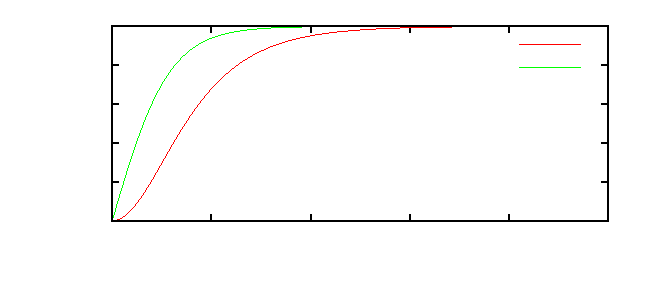
\includegraphics{f_and_h_funcs_monopole}}%
    \gplfronttext
  \end{picture}%
\endgroup

%  \caption{\em Numerical integration of the non-linear set of equation for
%    the 't~Hooft--Polyakov monopole. We have chosen $R=10$, $N=300$,
%    $\lambda v^2 = g^2v^2 = 1$.}
%  \label{fig:monopole}
%\end{figure}

\begin{subsection}{Energy functionnal}
  The mass (or energy) of the monopole is one of the quantity which
  can be estimated analytically. We can show the the mass only depends
  upon the ratio of the two free parameters of the Lagrangian:
  \begin{equation}
    E \sim \frac{v}{g}.
  \end{equation}
  Introducing a non-Minkowskian metric $g_{\mu\nu}$, the symmetric
  energy-momentum tensor writes:
  \begin{equation}
    \delta_{g_{\mu\nu}}S = \frac{1}{2}\int\mathrm{d}^4x\sqrt{-g}\bar T^{\mu\nu}\delta g_{\mu\nu}.
  \end{equation}
  We easily find that for the Lagrangian (\ref{eq:GGlagrangian}), the
  corresponding $\bar T^{\mu\nu}$ is
  \begin{equation}
    \bar T_{\mu\alpha} = -F_{\mu\nu}F_{\alpha}^{\hphantom{\alpha}\nu}+\mathrm{D}_\mu \phi^a \mathrm{D}_\alpha\phi^a-\eta_{\mu\alpha}\mathcal L.
  \end{equation}
  For a static configuration of the fields, the $\bar T_{00}$
  component reduces to
  \begin{equation}
    \bar T_{00} = \frac{1}{2}F_{0i}F_{0i}+\frac{1}{4}F_{ij}F_{ij} +\frac{1}{2}\mathrm{D}_0\phi^a\mathrm{D}_0\phi^a+\frac{1}{2}\mathrm{D}_i\phi^a\mathrm{D}_i\phi^a+\frac{\lambda}{4}\left(\phi^a\phi^a-v^2\right)^2
  \end{equation}
  Considering the 't Hooft Polyakov ansatz (\ref{eq:ansatz}), the
  expression reduce even further, and the energy functionnal reads:
  \begin{equation}
    E = 4\pi\int_0^\infty r^2\mathrm dr\left(\frac{1}{4}F_{ij}F_{ij}+\frac{1}{2}\mathrm{D}_i\phi^a\mathrm{D}_i\phi^a+\frac{\lambda}{4}\left(\phi^a\phi^a-v^2\right)^2\right).\label{eq:staticefunc}
  \end{equation}
  In terms of $f$ and $h$, it becomes:
  \begin{multline}
    E = \frac{4\pi}{g^2}\int_0^\infty \mathrm{d}r \left[f'^2+\frac{f^2(f-2)^2}{2r^2}+\frac{v^2g^2}{2}r^2h'^2\right.\\
      \left.+ v^2g^2h^2(1-f)^2+\frac{\lambda}{4}v^4g^2r^2(h^2-1)^2\right].\label{eq:efunc}
  \end{multline}
  Proceeding to the following change of variable:
  \begin{equation}
    f(r)=1-F(r);\quad h(r)=\frac{H(r)}{r} ;\quad \xi = gvr.
  \end{equation}
  The energy functional can be recast into
  \begin{equation}
    E = \frac{4\pi v}{g} C\left(\frac{\lambda}{g^2}\right)
  \end{equation}
  We note that that the minimization of the energy functional
  (\ref{eq:efunc}) with respect to $f$ and $h$ lead to the same field
  equations as (\ref{eq:monopole1})-(\ref{eq:monopole2}). 
  

  Given the numerical approximations for $f$ and $h$ found in previous
  section, we can estimate the energy in the following way:
  \begin{equation}
    \int_0^\infty \mathcal{E}(r, f, f', h, h')\mathrm d r \ \to\ \Delta\sum_{i = 1}^N \mathcal{E}\left(r_i, f_i, \frac{f_{i+1}-f{i-1}}{\Delta}, h_i, \frac{h_{i+1}-h_{i-1}}{\Delta}\right)
  \end{equation}
  where $\mathcal{E}$ is the energy density.
\end{subsection}

\end{section}
